
\subsection{Datasets}  
For analysing our versions of BAL \ref{sec:models-bal} we have chosen three datasets on which we tested and compared the performance of our models. 

\subsubsection{4-2-4 Encoder} 
\label{sec:datasets-auto4}


The \emph{4-2-4 econder} task is the simplest dataset we have been working with. It consists of four four--dimensional samples $(1,0,0,0)$, $(0,1,0,0)$, $(0,0,1,0)$ and $(0,0,0,1)$ which are each mapped to itself. We use two units on the hidden layer what gives us the 4-2-4 architecture. The 4-2-4 encoder task is a well--known problem and used previously for testing GeneRec \citep{o1996bio} and BAL \citep{farkas2013bal}. In the case of BAL only 60--65\% \emph{patSucc} was achieved which leaves a gap for improvement. Also this dataset as it's convenient for testing novel approaches as the learning progress of the network could be checked by hand and eye. 

%TODO consider \subsubsection{Simple Binary Vector Associations} 

\subsubsection{Complex Binary Vector Associations} 
\label{sec:datasets-k3}

The \emph{complex binary vector associations} task was used in \citet{farkas2013bal} and its motivated by the sensory--motor mappings between distributed patterns \citep{farkas2013bal}. The task is to associate sixteen 16--dimensional vectors all with 3 active units. There are always 4 distinct overlapping input patterns associated with exactly one output pattern. As the association is not unique in the \emph{backward} way it's impossible to achieve perfect $\mbox{bitSucc}^B$ or $\mbox{patSucc}^B$. Therefore we would expect from the network to gives a \emph{blend} of the four input patterns corresponding the one output. 

\begin{figure}[h]
  \centering
  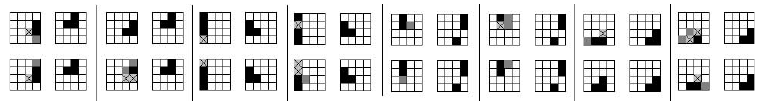
\includegraphics[width=0.8\textwidth]{img/cbva_back_repre.png} 
  \caption{BAL performance on complex binary vector associations: active units are filled with color, black = target–estimate match, gray = target only, gray with a cross = false-positive estimate \citep{farkas2013bal}.}
  \label{fig:datasets-k3}
\end{figure}

%tail -n +2 train.csv | sed 's/,/ /g' | awk 'BEGIN{FS=" "}{for(i=2;i<=NF;i++) {printf "%f ", $i / 256.0} printf "\n"}' >> buf.in
%echo "38000 784" > digits.in
%echo "4000 784" > digits.test.in
%tail -n +2 train.csv | sed 's/,/ /g' | awk 'BEGIN{FS=" "}{for(i=0;i<=9;i++) printf("%d ", $1 == i ? 1 : 0); printf "\n"}' > buf.out
%echo "38000 10" > digits.out
%echo "4000 10" > digits.test.out
%head -38000 buf.in >> digits.in 
%tail -4000 buf.in >> digits.test.in 
%head -38000 buf.out >> digits.out
%tail -4000 buf.out >> digits.test.out
%rm buf.* 
\subsubsection{Hand--written Digits} 
\label{sec:datasets-digits} 

The well--known MNIST dataset of \emph{Hand--written Digits} analysed by \citet{lecun1998gradient} and others (TODO cite) consists of 42,000 $28 \times 28$ grayscale images mapped to ten classes each representing one digit. We have chosen this dataset for three reasons. First, it's big and complex enough to test the practicallity of our models. Second, performance of many models (TODO ref: \url{http://yann.lecun.com/exdb/mnist/}) is known on this dataset and therefore we can easily compare performance of our models to these models. And third, we can easily visualize (TODO ref) the backward \emph{blend} representations and intuitively see if our models perform well. 

